%\documentclass[iop]{emulateapj}
\documentclass[aps, prl, twocolumn, nofootinbib, groupedaddress, amsfonts, amssymb, amsmath]{revtex4-1}
\usepackage{graphicx}
\usepackage{bm}
\usepackage{natbib}
%\usepackage[colorlinks=True, linkcolor=blue, citecolor=blue]{hyperref}
%\usepackage[all]{hypcap}

\bibliographystyle{apsrev}

\newcommand{\Div}[1]{\ensuremath{\nabla\cdot\left( #1\right)}}
\newcommand{\angles}[1]{\ensuremath{\left\langle #1 \right\rangle}}
\newcommand{\grad}{\ensuremath{\nabla}}
\newcommand{\RB}{Rayleigh-B\'{e}nard }
\newcommand{\stressT}{\ensuremath{\bm{\bar{\bar{\Pi}}}}}
\newcommand{\lilstressT}{\ensuremath{\bm{\bar{\bar{\sigma}}}}}
\newcommand{\nrho}{\ensuremath{n_{\rho}}}
\newcommand{\approptoinn}[2]{\mathrel{\vcenter{
	\offinterlineskip\halign{\hfil$##$\cr
	#1\propto\cr\noalign{\kern2pt}#1\sim\cr\noalign{\kern-2pt}}}}}

\newcommand{\appropto}{\mathpalette\approptoinn\relax}

\newcommand\mnras{{MNRAS}}%
          % Monthly Notices of the RAS

\begin{document}
%%%%% Create nice title and abstract
\author{Evan H. Anders}
\affiliation{Department of Astrophysical \& Planetary Sciences, University of Colorado -- Boulder}
\affiliation{Laboratory for Atmospheric and Space Physics, Boulder, CO}
\author{Benjamin P. Brown}
\affiliation{Department of Astrophysical \& Planetary Sciences, University of Colorado -- Boulder}
\affiliation{Laboratory for Atmospheric and Space Physics, Boulder, CO}
\title{Convective heat transport in stratified atmospheres at low and high Mach number}

\begin{abstract}
Convection in astrophysical systems is stratified and
often occurs at high Rayleigh number (Ra) and low
Mach number (Ma).
Here we study stratified convection in the context of 
plane-parallel, polytropically stratified atmospheres. 
We hold the density stratification ($n_{\rho}$) and Prandtl 
number (Pr) constant while varying the superadiabaticity
and Ra.  We find that Ma is primarily controlled by the
superadiabaticity of the atmosphere.  We also examine
the behavior of the Nusselt number (Nu), 
which quantifies the efficiency of convective heat transport,
and the Reynolds number (Re), which quantifies how turbulent our
solutions are.
%As Ra increases and $\text{Ma} \rightarrow 1$, a scaling 
%of Nu $\propto$ Ra$^{0.45}$ is observed.  
%As Ra increases to a regime where Ma $\geq 1$,
%this scaling gives way to a weaker Nu $\propto$ Ra$^{0.19}$. 
%In the regime of Ma $\ll 1$, a consistent
%Nu $\propto$ Ra$^{0.31}$ is retrieved,  reminiscent of the 
%Nu $\propto$ Ra$^{2/7}$ seen in \RB convection.
\end{abstract}
\maketitle


%%%%% Body of the paper
\section{Introduction}
\refstepcounter{section}
\label{sec:intro}
Convection transports energy in stellar and planetary atmospheres.
In these objects, flows are compressible and
feel the atmospheric stratification.  While in some systems this stratification 
is negligible, it is significant in regions such as
the convective envelope of the Sun, which spans 14 density scale heights.
In the bulk of these systems, flows are at very low Mach Number (Ma), 
but numerical constraints have restricted most studies of 
compressible convection to high Ma.
These studies have provided important insight into the low temperature, 
high Ma region near the Sun's surface, but few fundamental
properties of low Ma convection which characterize deeper motions
are known.

%Convective heat transport is essential
%in the cores of high mass stars,
%the envelopes of low mass stars, and the atmospheres of terrestrial and 
%jovian planets.  These astrophysical systems have density stratifications
%ranging from a few density scale heights (e.g. massive star cores)
%up to 14 density scale heights in the convective envelopes of low
%mass stars such as the Sun.
%Atmospheric stratification presumably modifies the fundamental
%dynamics and heat transport mechanisms of these atmospheres.
%Understanding the fundamental
%properties of compressible convection in stratified media is essential
%to characterizing systems in astrophysics and planetary sciences.  
%Numerical constraints have often restricted studies of compressible
%convection to moderately high Mach number (Ma), appropriate to regions near 
%the Sun's surface.  Few fundamental properties of
%low Ma convection, which occurs in the deep solar interior, are known.

In the widely-studied \RB (RB) problem of Boussinesq convection, 
upflows and downflows are symmetrical and
the conductive flux ($\propto \grad T$) approaches 
zero in the convective interior.
Early numerical experiments of moderate-to-high Ma compressible convection
in two \cite{graham1975, chan&all1982,
hurlburt&all1984, cattaneo&all1990} and three 
\cite{cattaneo&all1991, brummell&all1996} dimensions
revealed that these two hallmark characteristics of RB convection change
significantly when stratification is included.  Downflow lanes
become fast and narrow, and upflow lanes turn into broad, slow upwellings.
Furthermore, the \emph{entropy} gradient is negated by convection 
rather than the temperature gradient, and
a significant conductive flux can exist in the presence of
efficient convection.

In RB convection, there exist two primary dynamical control parameters: 
the Rayleigh number (Ra, the ratio of
buoyant driving to diffusive damping) and the Prandtl number 
(Pr, the ratio of viscous to thermal
diffusivity). These numbers control two useful
measures of turbulence in the evolved solution:
the Reynolds
number (Re, the strength of advection to viscous diffusion)
and the Peclet number (Pe = Re Pr).  Stratified atmospheres
with negative entropy gradients are unstable to convection.
The magnitude of the unstable entropy gradient, or the superadiabaticity,
joins Ra and Pr as an important control parameter.  This 
\emph{superadiabatic excess} \cite{graham1975}, $\epsilon$, which 
sets the scale of the atmospheric entropy gradient,
primarily controls the Ma of the evolved solution.

%In RB convection, there exist two primary control parameters: 
%the Rayleigh number (Ra, the ratio of
%buoyant driving to diffusive damping) and the Prandtl number 
%(Pr, the ratio of viscous to thermal
%diffusivity).  These numbers coupled with the aspect ratio of 
%the physical domain and the boundary conditions
%determine the dynamics of the convection.  In stratified atmospheres, 
%in addition to specifying the equation of state and
%fundamental properties of the gas, the two control parameters of 
%RB convection are joined by the degree of
%stratification across the domain and the characteristic 
%Ma of the convective flows.  
%Polytropically stratified atmospheres, such as those used in 
%early studies \cite{graham1975, chan&all1982, hurlburt&all1984, 
%cattaneo&all1990, cattaneo&all1991, brummell&all1996}, are an ideal extension of
%RB convection into the stratified realm because the two additional 
%control parameters are directly linked to
%basic properties of the atmosphere.  The density stratification is 
%set by the number of density scale heights (\nrho)
%the atmosphere spans, and Ma is controlled 
%by the superadiabatic excess ($\epsilon$),
%the deviation of the polytropic index from the adiabatic polytropic 
%index \cite{graham1975}.

In this letter we study the behavior of convective heat transport, 
quantified by the Nusselt number (Nu), in plane-parallel, 
two-dimensional, polytropically stratified atmospheres.  
We vary $\epsilon$ and Ra while holding Pr, aspect ratio, boundary conditions,
and initial atmospheric stratification
constant.  We describe experimental methods in section 
\ref{sec:experiment}, including the construction of atmospheres, 
equations, and numerical methods.  
Results are described in section \ref{sec:results} 
and their implications are discussed
in section \ref{sec:discussion}.

\section{Experiment} 
\refstepcounter{section}
\label{sec:experiment}
We examine a monatomic ideal gas with an adiabatic index of
$\gamma = 5/3$ whose equation of state is $P = R\rho T$.
This is consistent with the approach used in earlier work
and is the simplest stratified extension of RB.
We study atmospheres which are initially polytropically stratified,
\begin{equation}
\begin{split}
\rho_0(z) &= \rho_{t}(1 + L_z - z)^m, \\
T_0(z)    &= T_{t}(1 + L_z - z),
\label{eqn:polytrope}
\end{split}
\end{equation}
where $m$ is the polytropic index and $L_z$ is the depth of the atmosphere.
The height coordinate, $z$, increases upwards in the range $[0, L_z]$.  We
specify the depth of the atmosphere, $L_z = e^{n_{\rho}/m} - 1$, by choosing
the number of density scale heights, $n_{\rho}$, it spans.
Throughout this letter we set $n_{\rho} = 3$.  Satisfying hydrostatic
equilibrium sets the value of gravity, $g = R T_t (m + 1)$, which is
constant with depth.  We study two-dimensional atmospheres with aspect
ratios of 4 where the $x$ coordinate has the range $[0, 4L_z]$.

%
%We examine the simplest stratified extension of RB by studying a
%fluid composed of monatomic ideal gas particles with an adiabatic 
%index of $\gamma = 5/3$ and whose equation of state is $P = R\rho T$. 
%This is consistent with the approach used in earlier work.
%The initial atmosphere is a plane-parallel polytrope in which 
%the gravitational acceleration and conductive flux, 
%$\bm{F}_{\text{cond,0}} = -\kappa \partial_z T_0$, do not vary with depth. To
%achieve the latter condition, both $\kappa$ and $\partial_z T_0$ are constant.
%Under these assumptions, satisfying hydrostatic 
%equilibrium produces a stratification of
%\begin{equation}
%\begin{split}
%\rho_0(z) &= \rho_{t}(z_0 - z)^m, \\
%T_0(z)    &= T_{t}(z_0 - z),
%\label{eqn:polytrope}
%\end{split}
%\end{equation}
%where $m = m_{\text{ad}} - \epsilon$ is the polytropic index.
%The adiabatic polytropic index is $m_{\text{ad}} \equiv (\gamma-1)^{-1}$, and
%the superadiabatic excess is $\epsilon$ which sets the scale 
%of the entropy gradient ($\partial_z S_0 \propto -\epsilon$).
%A significant advance of this work is the ability to study large 
%and small values of $\epsilon$, as will be discussed.
%Thermodynamic variables are nondimensionalized at the 
%top of the atmosphere as  $P_0(L_z) = \rho_0(L_z) = T_0(L_z) = 1$, 
%requiring $z_0 \equiv L_z + 1$ and $R = T_{t} = \rho_{t} = 1$.
%By this choice, the non-dimensional length scale is the inverse 
%temperature gradient scale and the timescale is the isothermal 
%sound crossing time of this unit length.
%The height $z$ increases upwards within $[0, L_{z}]$, 
%where $L_{z} = e^{n_{\rho}/m} - 1$ is
%determined by $n_\rho$ and $\epsilon$.
%The characteristic timescale of convective dynamics
%is related to the atmospheric buoyancy time, 
%$t_{\text{b}} = \sqrt{L_z/g\epsilon}$, with $g = (m+1)$.
%Throughout this letter, we use buoyancy time units and 
%choose $n_{\rho} = 3$ such that the 
%initial density varies by a factor of 20.
%All atmospheres studied here have an aspect ratio of 4, 
%such that $L_x = 4L_z$.
%

Convective dynamics are controlled by the superadiabaticity
of the atmospheres as well as the atmospheric diffusivities.
The superadiabaticity, or the magnitude of the (negative) 
entropy gradient, is set by 
the superadiabatic excess, $\epsilon = m_{ad} - m$, where 
$m_{ad} = (\gamma - 1)^{-1}$.
The atmospheric thermal diffusivity, $\chi$,
and kinematic viscosity (or viscous diffusivity), $\nu$,
are determined by the Rayleigh number (Ra) and the Prandtl
number (Pr).  We set $\text{Pr } = \nu/\chi = 1$ throughout
this work. The polytropic initial conditions are in
thermal equilibrium, $\kappa_0 \partial_z T_0 =$ const,
so $\kappa_0 = \chi \rho_0$ must be constant. To keep
Pr constant with height, we set $\chi = \chi_t/\rho_0$
and $\nu = \nu_t/\rho_0$.  Under these constraints, the
diffusivity profiles are specified by choosing Ra
at the top of the domain,
\begin{equation}
\text{Ra}_{\text{top}} = \frac{g L_z^3 (\Delta S_0 / c_P)}{\nu_t\chi_t},
\end{equation}
where $\Delta S_0 = \epsilon\ln z_0$ is the entropy difference 
between the top and bottom boundaries and
$c_P = R\gamma(\gamma-1)^{-1}$ is the specific heat 
at constant pressure. The profiles of $\nu$ and $\chi$ are constant with
time, and Ra at the bottom of the atmosphere is greater than Ra$_{\text{top}}$
by a factor of $e^{2n_{\rho}}$.  This formulation leaves
the thermal conductivity, $\kappa = \rho\chi$, and
the dynamic viscosity, $\mu = \rho\chi$, free to evolve
as the density profile changes.

We decompose our thermodynamic variables such that $T = T_0 + T_1$ and
$\ln\rho = (\ln\rho)_0 + (\ln\rho)_1$, 
and the velocity $\bm{u} = u\hat{x} + w\hat{z}$ 
has no background component.    
We evolve the Fully Compressible Navier-Stokes equations,
\begin{align}
&\begin{aligned}
&\frac{\partial \ln\rho}{\partial t} + \grad\cdot\bm{u} 
    = -\bm{u}\cdot\grad\ln\rho,
	\label{eqn:continuity_eqn}
\end{aligned}\\
&\begin{aligned}
\frac{\partial\bm{u}}{\partial t} + \grad T - 
&\nu\grad\cdot\lilstressT - \lilstressT\cdot\grad\nu = \\
&-\bm{u}\cdot\grad\bm{u} - T\grad\ln\rho + \bm{g} + 
\nu\lilstressT\cdot\grad\ln\rho,
\label{eqn:momentum_eqn}
\end{aligned}\\
&\begin{aligned}
\frac{\partial T}{\partial t} -\frac{1}{c_V}\left(\right.\chi&\left.
    \grad^2 T + \grad T\cdot\grad\chi\right) = \\
	&-\bm{u}\cdot\grad T - (\gamma-1)T\grad\cdot{\bm{u}} \\
	&+ \frac{1}{c_V}\left(\chi\grad T \cdot\grad\ln\rho +
	\nu\left[\lilstressT\cdot\nabla\right]\cdot\bm{u}\right), 
	\label{eqn:energy_eqn}
\end{aligned}
\end{align}
with the viscous stress tensor given by
\begin{equation}
\sigma_{ij} \equiv \left(\frac{\partial u_i}{\partial x_j} + 
\frac{\partial u_j}{\partial x_i} - \frac{2}{3}\delta_{ij}\grad\cdot\bm{u}\right).
	\label{eqn:stress_tensor}
\end{equation}
Taking an inner product of
(\ref{eqn:momentum_eqn}) with $\bm{u}$ and adding it to 
(\ref{eqn:energy_eqn}) reveals the full energy equation,
\begin{equation}
\frac{\partial}{\partial t}\left(\rho\left[\frac{|\bm{u}|^2}{2} + c_V T + \phi\right]\right) +
\Div{\bm{F}_{\text{conv}} + \bm{F}_{\text{cond}}} = 0,
	\label{eqn:energy_eqn_full}
\end{equation}
where
$
\bm{F}_{\text{conv}} \equiv \bm{F}_{\text{enth}} + \bm{F}_{\text{KE}} + \bm{F}_{\text{PE}} + \bm{F}_{\text{visc}}
$
is the convective flux and $\bm{F}_{\text{cond}} = -\kappa \grad T$
is the conductive flux.
The individual contributions to $\bm{F}_{\text{conv}}$ are the enthalpy flux, 
$\bm{F}_{\text{enth}} \equiv \rho\bm{u}(c_V T + P/\rho)$;
the kinetic energy flux, 
$\bm{F}_{\text{KE}} \equiv \rho|\bm{u}|^2\bm{u}/2$;
the potential energy flux,
$\bm{F}_{\text{PE}} \equiv \rho\bm{u}\phi$ (with $\phi \equiv -gz$);
and the viscous flux, 
$\bm{F}_{\text{visc}} \equiv -\rho\nu\bm{u}\cdot\lilstressT$, and each 
must be considered. 
Understanding how these fluxes interact  
is crucial in characterizing convective heat transport.

We utilize the 
Dedalus\footnote{http://dedalus-project.org/} \cite{burns&all2016} 
pseudospectral framework to time-evolve  
(\ref{eqn:continuity_eqn})-(\ref{eqn:energy_eqn}) 
using an implicit-explicit (IMEX), third-order, four-step 
Runge-Kutta timestepping scheme RK443 \cite{ascher&all1997}.  
Variables are time-evolved on a dealiased Chebyshev (vertical)
and Fourier (horizontal, periodic) domain in which the
physical grid dimensions are 3/2 the size of the coefficient grid.  
Physical grid sizes range from
96x384 grid points at the lowest values of 
Ra to 1536x6144 grid points at Ra$_{\text{top}} > 10^{7}$. 
By using IMEX timestepping, we implicitly step the 
stiff linear acoustic wave contribution and are able to
efficiently study flows at moderate ($\approx 1$) 
and very low ($\approx 10^{-4}$) Ma.  Our equations take the form
of the FC equations in \cite{lecoanet&all2014}, extended to include
$\nu$ and $\chi$ which vary with depth, and we follow the approach there.
This IMEX approach has been successfully 
tested against a nonlinear benchmark  of the compressible 
Kelvin-Helmholtz instability \cite{Lecoanet_et_al_2016_KH}.

We impose impenetrable, stress free, fixed temperature boundary conditions at
the top and bottom of the domain such that 
$w = \partial_z u = T_1 = 0$ at $z = \{0, L_z\}$. 
$T_1$ is initially filled with
random white noise whose magnitude is infinitesimal
compared to $T_0$ and $\epsilon$.
We filter this noise spectrum in coefficient space, 
such that 25\% of the coefficients
have power. We non-dimensionalize our computational domains by setting
all thermodynamic variables to unity at $z = L_z$ by choosing
$R = T_t = \rho_t = 1$.  By this choice, the non-dimensional
grid length scale is the inverse temperature gradient scale and the 
simulation timescale is the isothermal sound crossing time, 
$\tau_I$, of this unit length.
Meaningful convective dynamics occur on 
timescales of the atmospheric buoyancy time,
$t_b = \tau_I \sqrt{L_z/g\epsilon}$, 
and all reported results are taken from time averages
over many buoyancy times starting 100$t_b$ 
after the start of our simulations in order to
assure our results are not biased by the convective transient.

\section{Results}
\refstepcounter{section}
\label{sec:results}


\begin{figure}[t]
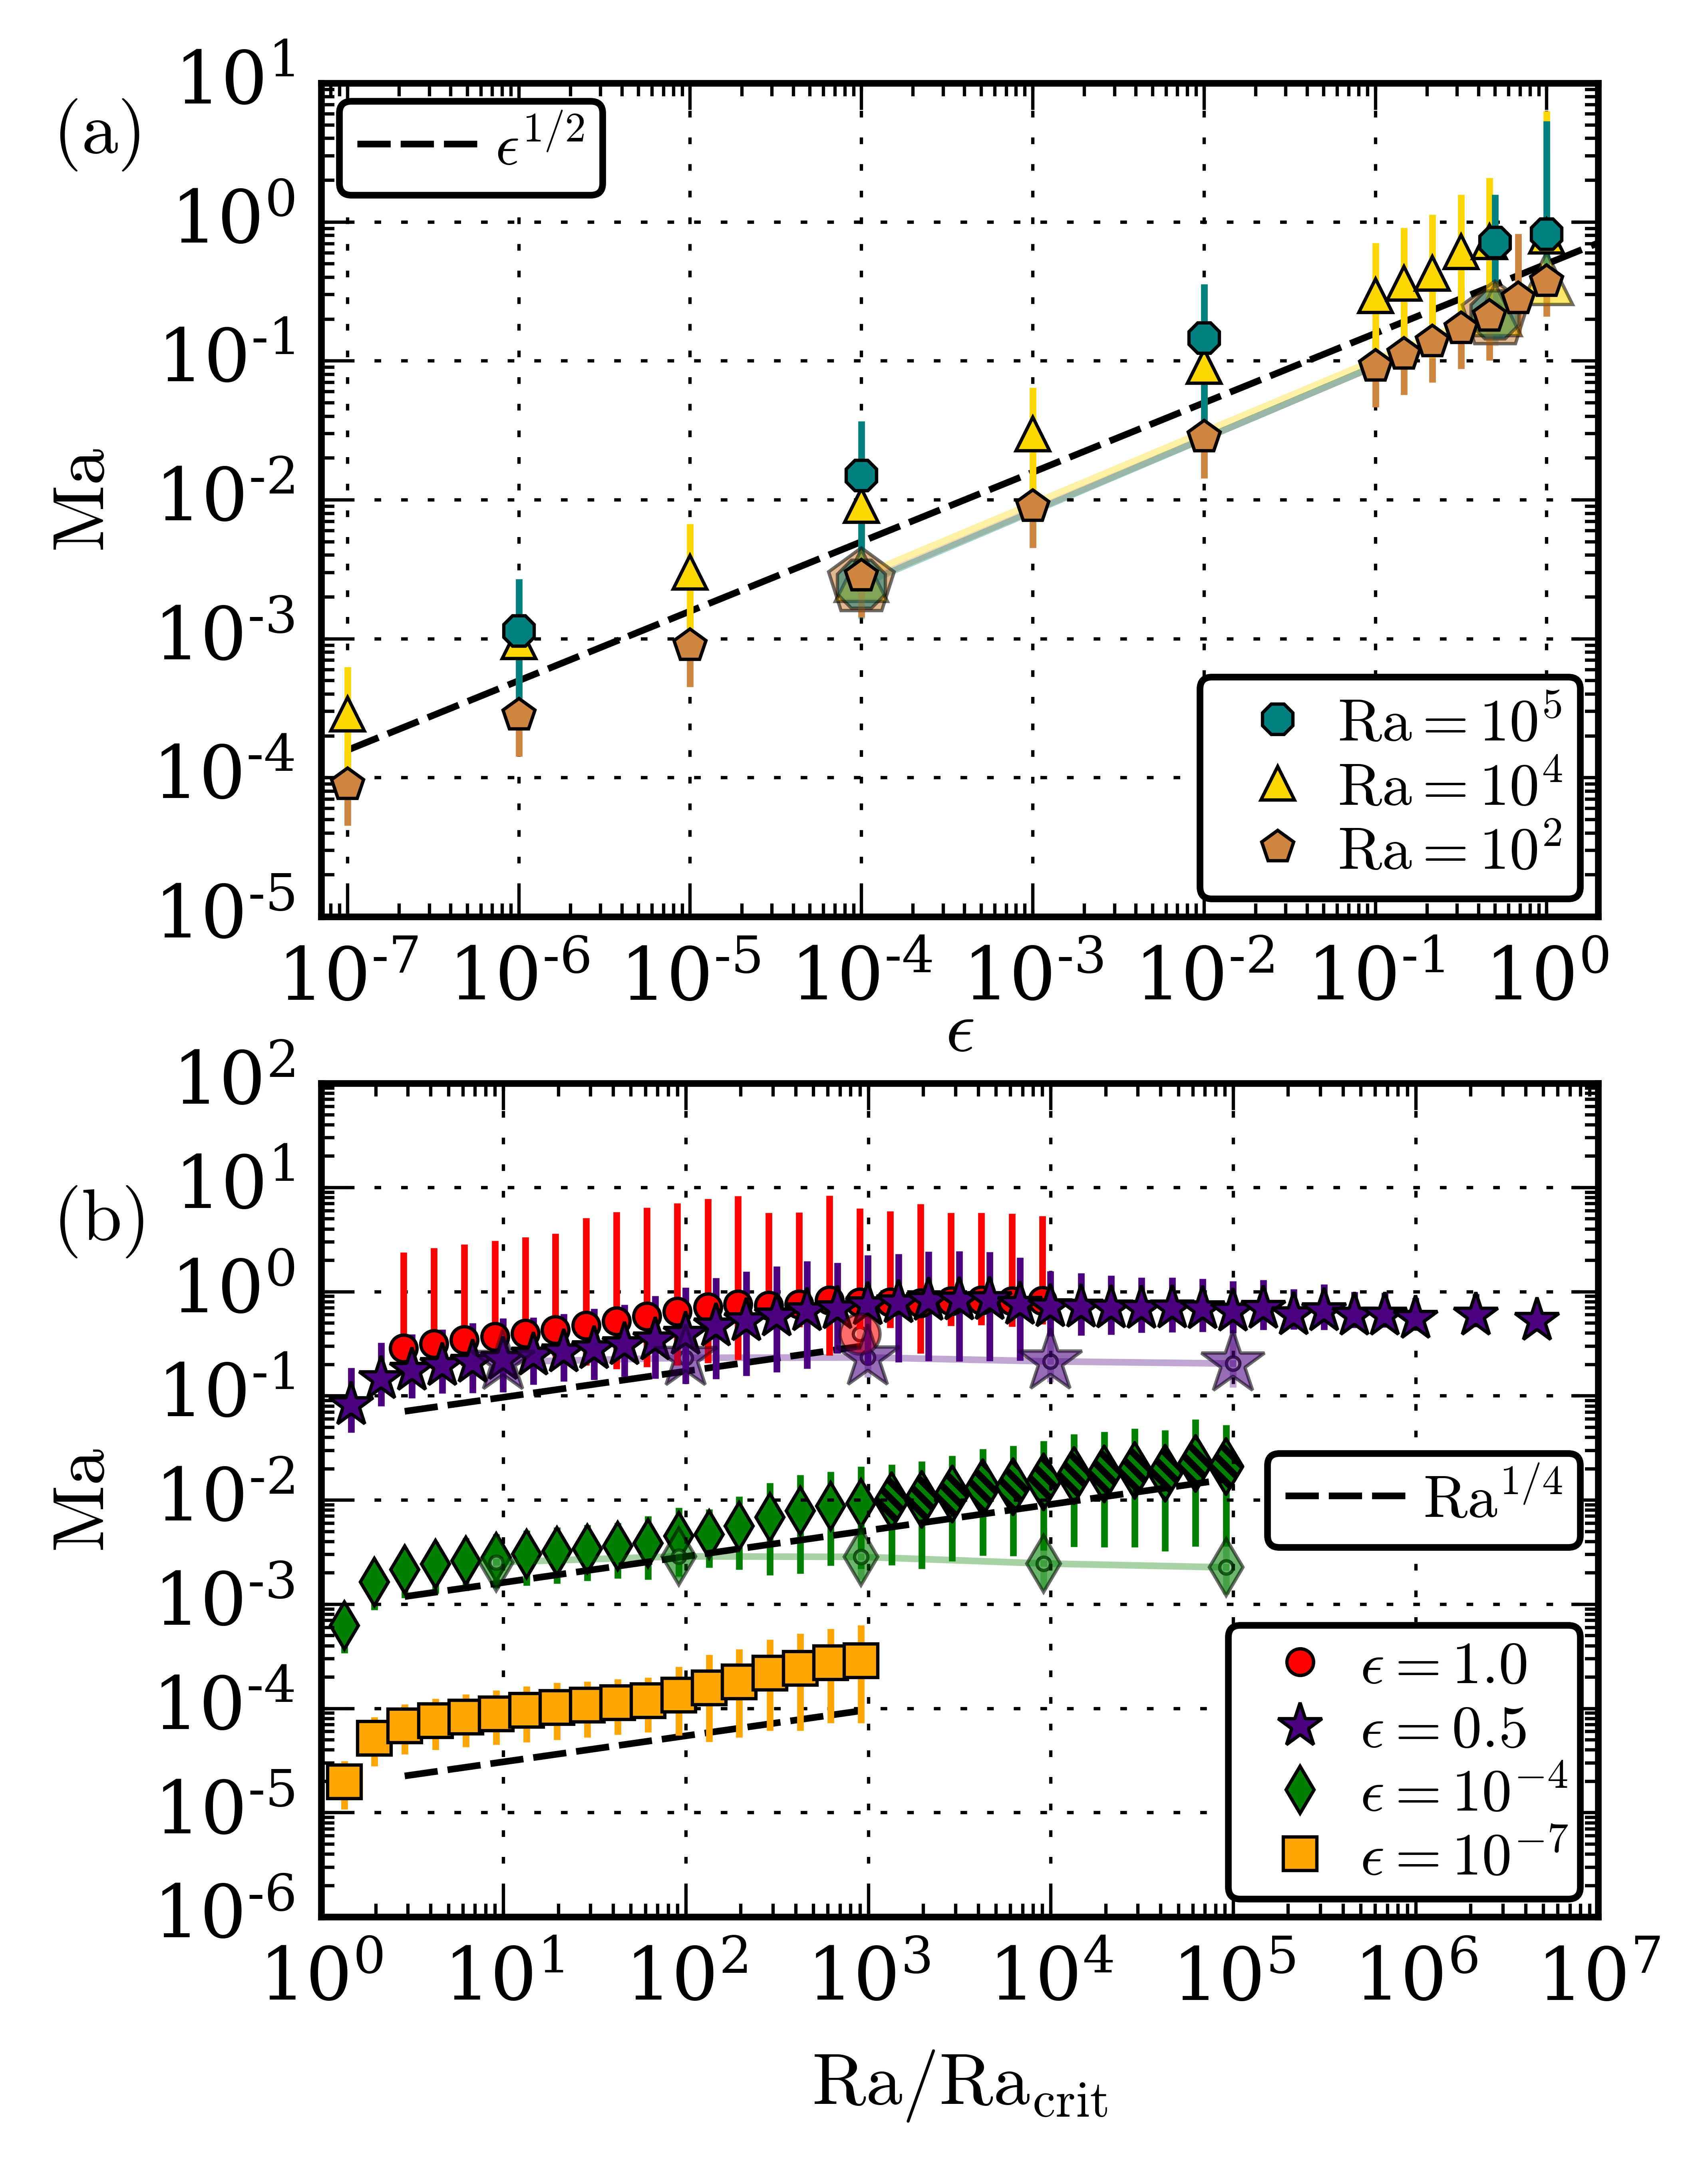
\includegraphics[width=3.4375in]{./figs/ma_v_Ra.png}
\caption{The mean adiabatic Mach number of long-time-averaged profiles
is shown.  Error bars show the full range of Ma over the depth of the
atmosphere.
(a) When $Ma < 1$ (below the black horizontal line), 
Ma $\propto \epsilon^{1/2}$.
t low ($10^2$) and moderate ($10^5$) values of Ra.
(b) When Ra is small, Ma $\propto Ra^{1/2}$ (dashed lines).
Once the mean Ma reaches 1 ($\epsilon = \{0.5, 1\}$), this scaling breaks down
and nearly all flows in the atmosphere are at Ma = 1.
At low $\epsilon$, a consistent power law of Ma $\propto Ra^{1/4}$ is retrieved.
\label{fig:ma_v_eps} }
\end{figure}


Solutions were time-evolved until a long time average of the fluxes
showed little
variance with depth. By performing a linear stability analysis, 
we determined that the onset of convection
occurs at $\text{Ra}_{\text{c,top}} = \{11.15, 10.06, 10.97, 10.97\}$ 
for $\epsilon = \{1.0, 0.5, 10^{-4}, 10^{-7}\}$ respectively.  
We studied Rayleigh
numbers from values at onset to values $\geq 10^6$Ra$_{\text{c,top}}$ 
for $\epsilon = 0.5$, up to
roughly $10^5$Ra$_{\text{c,top}}$ at $\epsilon = 10^{-4}$, and 
up to $10^3$Ra$_{\text{c,top}}$ for $\epsilon = \{1, 10^{-7}\}$.

We find that the Mach number is a strong function of 
$\epsilon$ and a weak function of Ra.  
When Ma $< 1$, Ma $\propto \epsilon^{1/2}$, 
but this relation break down as the mean
Ma approaches 1 and the flows become supersonic (see Fig. \ref{fig:ma_v_eps}a).  At low
Ra (Ra$_{\text{c,top}} \lesssim 10^4$), 
Ma $\propto$ Ra$^{1/4}$.  At high epsilon
($\epsilon = 0.5$, this scaling breaks down near 
Ra = $10^4$ where the flows become primarily
supersonic.  The scaling of 
Ra$^{1/4}$ appears to break down for Ra $\gtrsim 10^5$ at
$\epsilon = 10^{-4}$, 
but computational constraints made it restrictively difficult to converge
many runs in this region of parameter space.
Furthermore, the evolved thermodynamic variables, 
$T_1/T_0, \rho_1/\rho_0 \propto \epsilon$,
are very small for low Ma flows, 
but are order 1 when $\epsilon$ and Ma approach 1.

\begin{figure}[t]
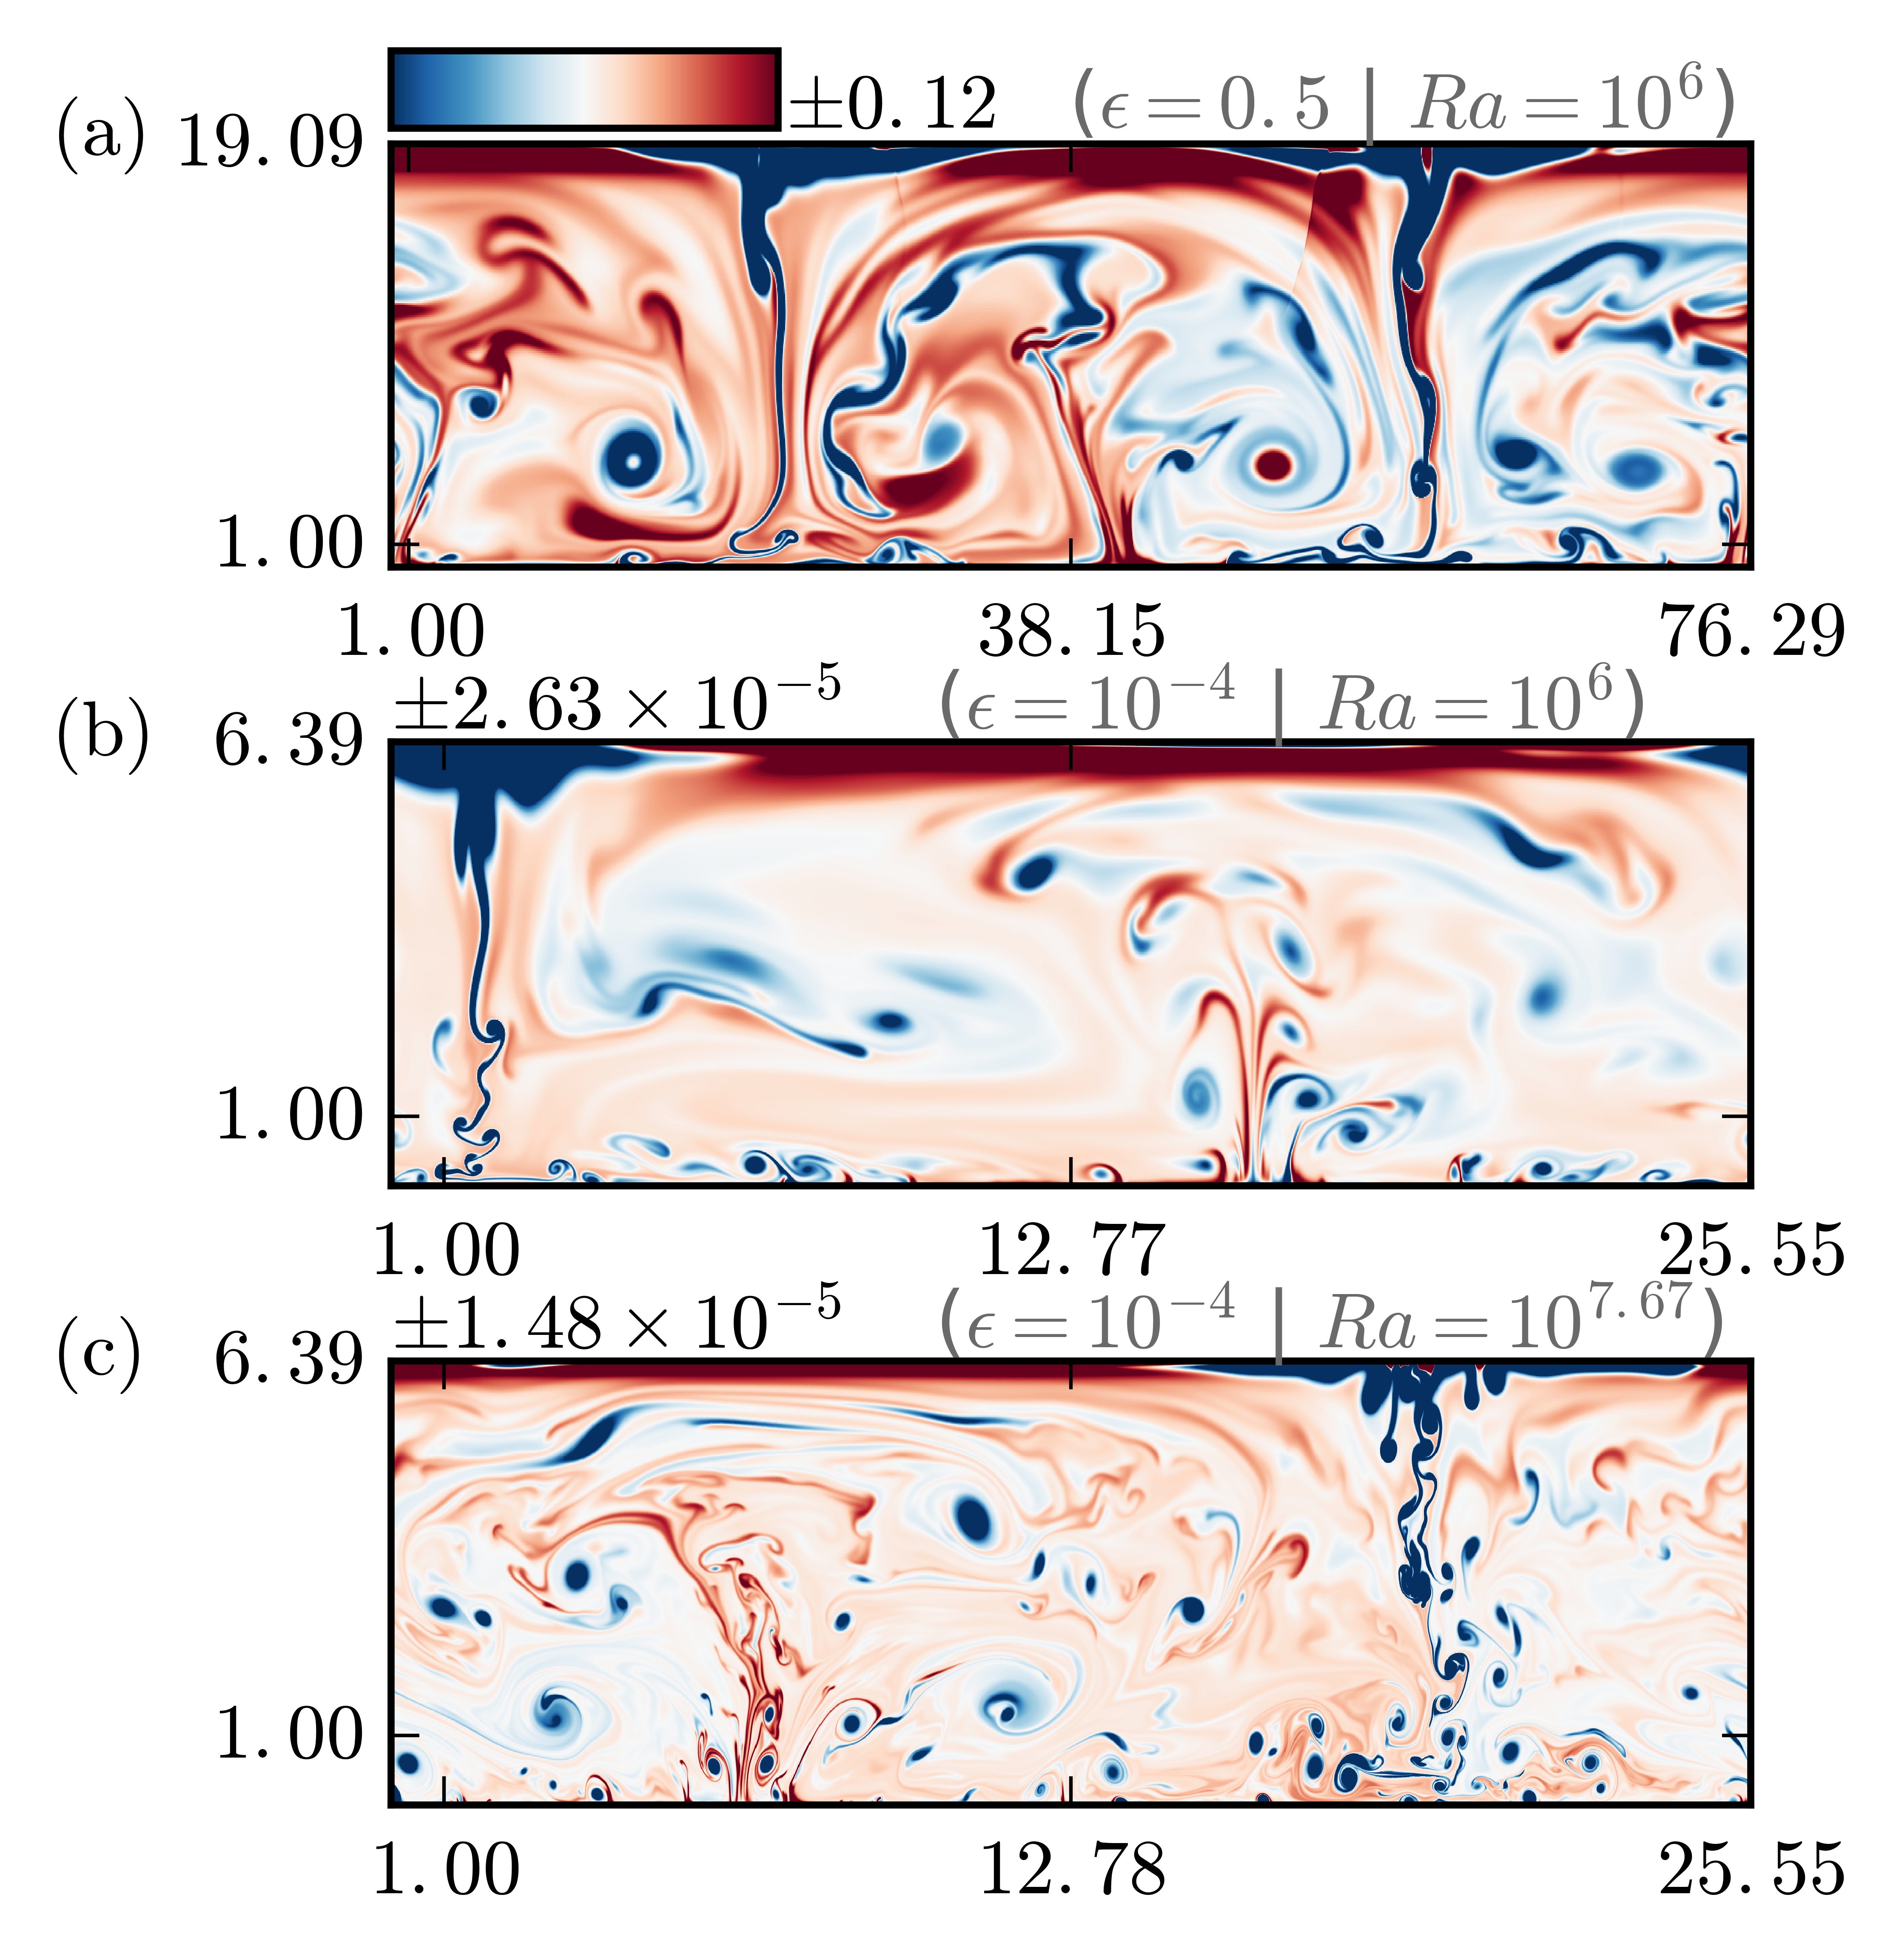
\includegraphics[width=3.4375in]{./figs/snapshots_fig.png}
\caption{Characteristic entropy fluctuations in evolved flows. 
The time- and horizontally-averaged profile is removed in all cases.  
(a) At high $\epsilon$, shock systems form near the upper downflow lanes 
($x \approx 45, z \approx 15-19$) at sufficiently high Ra.
Shock-heated fluid then flows into the downflows as the shocks propagate across upflows.
(b) At low $\epsilon$ but at the same Ra, shock systems are absent, 
but otherwise the dynamics are similar.  
(c) As Ra is increased, downflows no longer span
the entirety of the domain and individual 
small eddies are responsible for carrying the flux.
\label{fig:entropy_snapshots} }
\end{figure}

Low Ma flows ($\epsilon = 10^{-4}$)
display the classic narrow downflow and broad upflow lanes of stratified
convection (Fig. \ref{fig:entropy_snapshots}a).
While it has been suggested that pressure forces 
cause symmetry breaking in up- and downflows
\cite{hurlburt&all1984}, at low $\epsilon$ this 
effect seems to be secondary to flows obeying mass conservation as they traverse
the stratified medium.  
Our choice of fixed-temperature boundary conditions allows the flux at the 
boundaries to vary, and runs at $\text{Ra }> 10^4$
and $\epsilon = 10^{-4}$ exhibit long-term states of
flux disequilibrium.  
Roll solutions such as those pictured in Fig. \ref{fig:entropy_snapshots}a
are punctuated by states of vigorous shearing, similar to those previously
reported in two-dimensional RB convection \cite{goluskin&all2014}.  
During the roll states, 
the flux at the lower boundary exceeds that at the upper boundary
and energy is stored in the system.
During shearing states, 
convective transport is suppressed and Nu diminishes while
the flux at the upper boundary exceeds that at the lower boundary.  Long term
averages over both of these states produce flat flux profiles which
can be sensibly analyzed.

At large Ma ($\epsilon = 0.5$), bulk thermodynamic structures are similar but
shock systems form in the upper atmosphere near downflow lanes 
once Ra is sufficiently large  (Fig. \ref{fig:entropy_snapshots}b,c).
Similar shock phenomena were reported in
both two \cite{cattaneo&all1990} and 
three \cite{malagoli&all1990} dimensional polytropic simulations previously.
As Ra is increased to large values 
(Fig. \ref{fig:entropy_snapshots}c), thermodynamic structures 
no longer span the whole domain but rather break up into 
small eddies which traverse the domain multiple
times before diffusing.  

\begin{figure}[t]
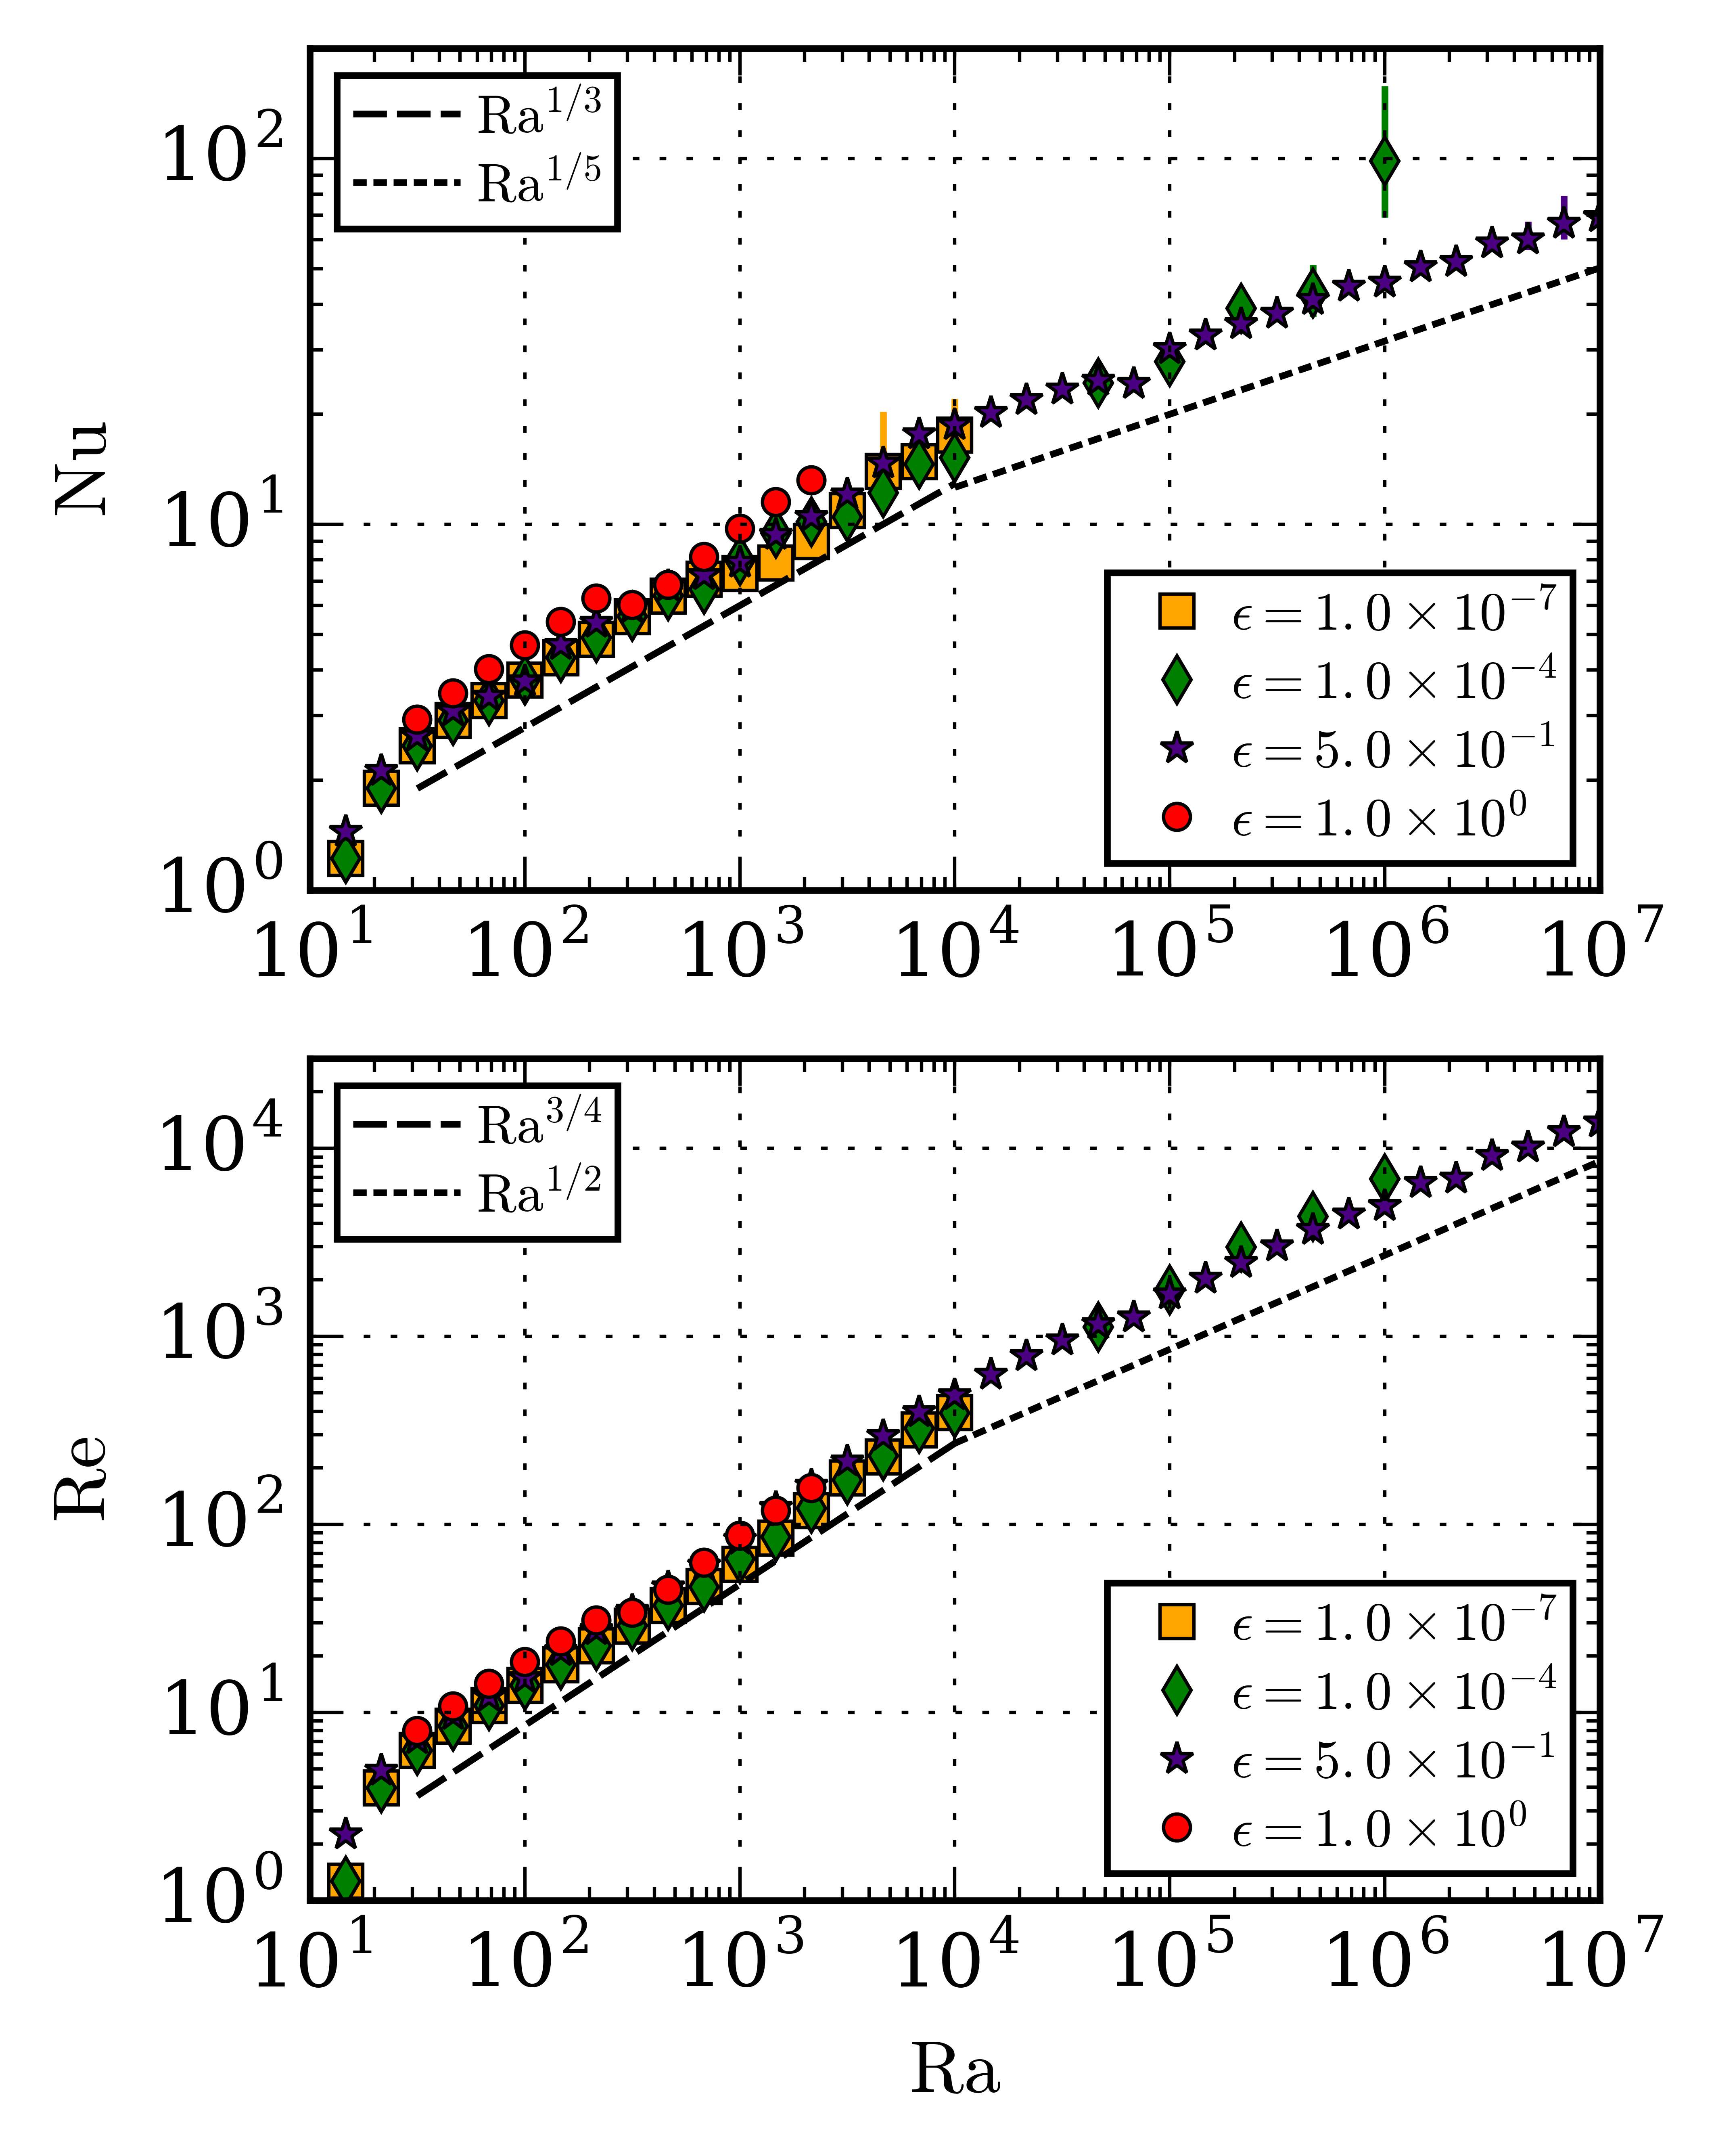
\includegraphics[width=3.4375in]{./figs/re_and_nu_v_Ra.png}
\caption{
Variation of Nu as Ra increases at high and low $\epsilon$. 
At high $\epsilon$ (purple circles), 
a clear transition from the subsonic to supersonic regime 
is evident in the scaling
of Nu with Ra at $\text{Ra}_{\text{top}} \approx 10^4$.  
In the low $\epsilon$ regime (green diamonds and yellow squares), 
our observed Nu scalings collapse onto a similar line which is
indistinguishable from a $\text{Ra}_{\text{top}}^{2/7}$ scaling, 
as observed in RB convection \cite{johnston&doering2009}.  
Errors bars indicate the properly normalized range of the
value of Nu as a function of depth and
large error bars indicate a poorly converged solution.
 \label{fig:re_and_nu_v_ra}.
}
\end{figure}

The efficiency of convection is quantified by the Nusselt number (Nu).  
Nu is well-defined in RB convection
as the total flux normalized by the steady-state conductive flux 
\cite{johnston&doering2009, otero&all2002}.
In stratified convection Nu is more difficult to define, and we use
a modified version of a traditional stratified Nusselt number 
\cite{graham1975,hurlburt&all1984},
\begin{equation}
\text{Nu} \equiv \frac{\langle F_{\text{conv,z}} + F_{\text{cond,z}} - F_{\text{A}}\rangle}
{\langle F_{\text{cond,z}} - F_{\text{A}}\rangle} 
= 1 + \frac{\langle F_{\text{conv,z}}\rangle}{\langle F_{\text{cond,z}} - F_{\text{A}} \rangle}
\label{eqn:nusselt}
\end{equation}
where $F_{\text{conv,z}}$ and $F_{\text{cond,z}}$ are the 
z-components of $\bm{F}_{\text{conv}}$ and $\bm{F}_{\text{cond}}$,
respectively and $\langle \rangle$ are volume averages.  
$F_{\text{A}} \equiv -\langle\kappa\rangle \partial_z T_{\text{ad}}$ 
is the conductive flux of the proper corresponding adiabatic atmosphere
with $\partial_z T_{\text{ad}} \equiv - g / c_{P}$ 
for a compressible ideal gas in hydrostatic equilibrium \cite{spiegel&veronis1960}.  Here we specify
$\langle \kappa \rangle = \langle \rho\chi \rangle$, which is nearly
$\kappa_0$ when $\epsilon$ is small but can change appreciably for large
values of $\epsilon$.
In incompressible Boussinesq convection, where $\grad S = 0$ only when 
$\grad T = 0$, this definition reduces to the traditional definition
of the Nusselt number \cite{otero&all2002, johnston&doering2009}.

The variation of Nu with Ra$_{\text{top}}$ is shown in 
Fig. \ref{fig:re_and_nu_v_ra}a.
At low to moderate Ra$_{\text{top}}$, 
Nu $\propto$ Ra$_{\text{top}}^{1/3}$ regardless of $\epsilon$,
as predicted by classical \RB theory \cite{king&all2012}.
At large Ra$_{\text{top}}$, Nu $\propto$ Ra$_{\text{top}}^{1/5}$ 
at $\epsilon = 0.5$.
The scaling of Nu with Ra$_{\text{top}}$ 
is unclear at low $\epsilon$ (so I'll try to fill in that space with
data from comps...time to fish it out of Lou and do post-processing hell).

The Reynolds number and Peclet number,
\begin{equation}
\text{Re} = \frac{|\bm{u}| L_z}{\nu};\,\,\,\,\text{Pe} = \text{Pr}\,\text{Re},
\end{equation}
quantify the importance of advection to diffusion in the evolved
convective state.  For Pr = 1, such as in this work, Pe = Re.  
Our choice of $\{\nu,\chi\}\propto \rho_0^{-1}$ drastically changes
the value of Re between the top and bottom of the atmosphere.  We report values of
Re at the midplane ($z=L_z/2$) of the atmosphere in
Fig. \ref{fig:re_and_nu_v_ra}b.
At low Ra$_{\text{top}}$, Re $\propto$ Ra$_{\text{top}}^{3/4}$, but at high 
Ra$_{\text{top}}$ where the average Ma $\approx 1$ for $\epsilon = 0.5$, 
this scaling gives way to a Re $\propto$ Ra$_{\text{top}}^{1/2}$.

\begin{figure}[t]
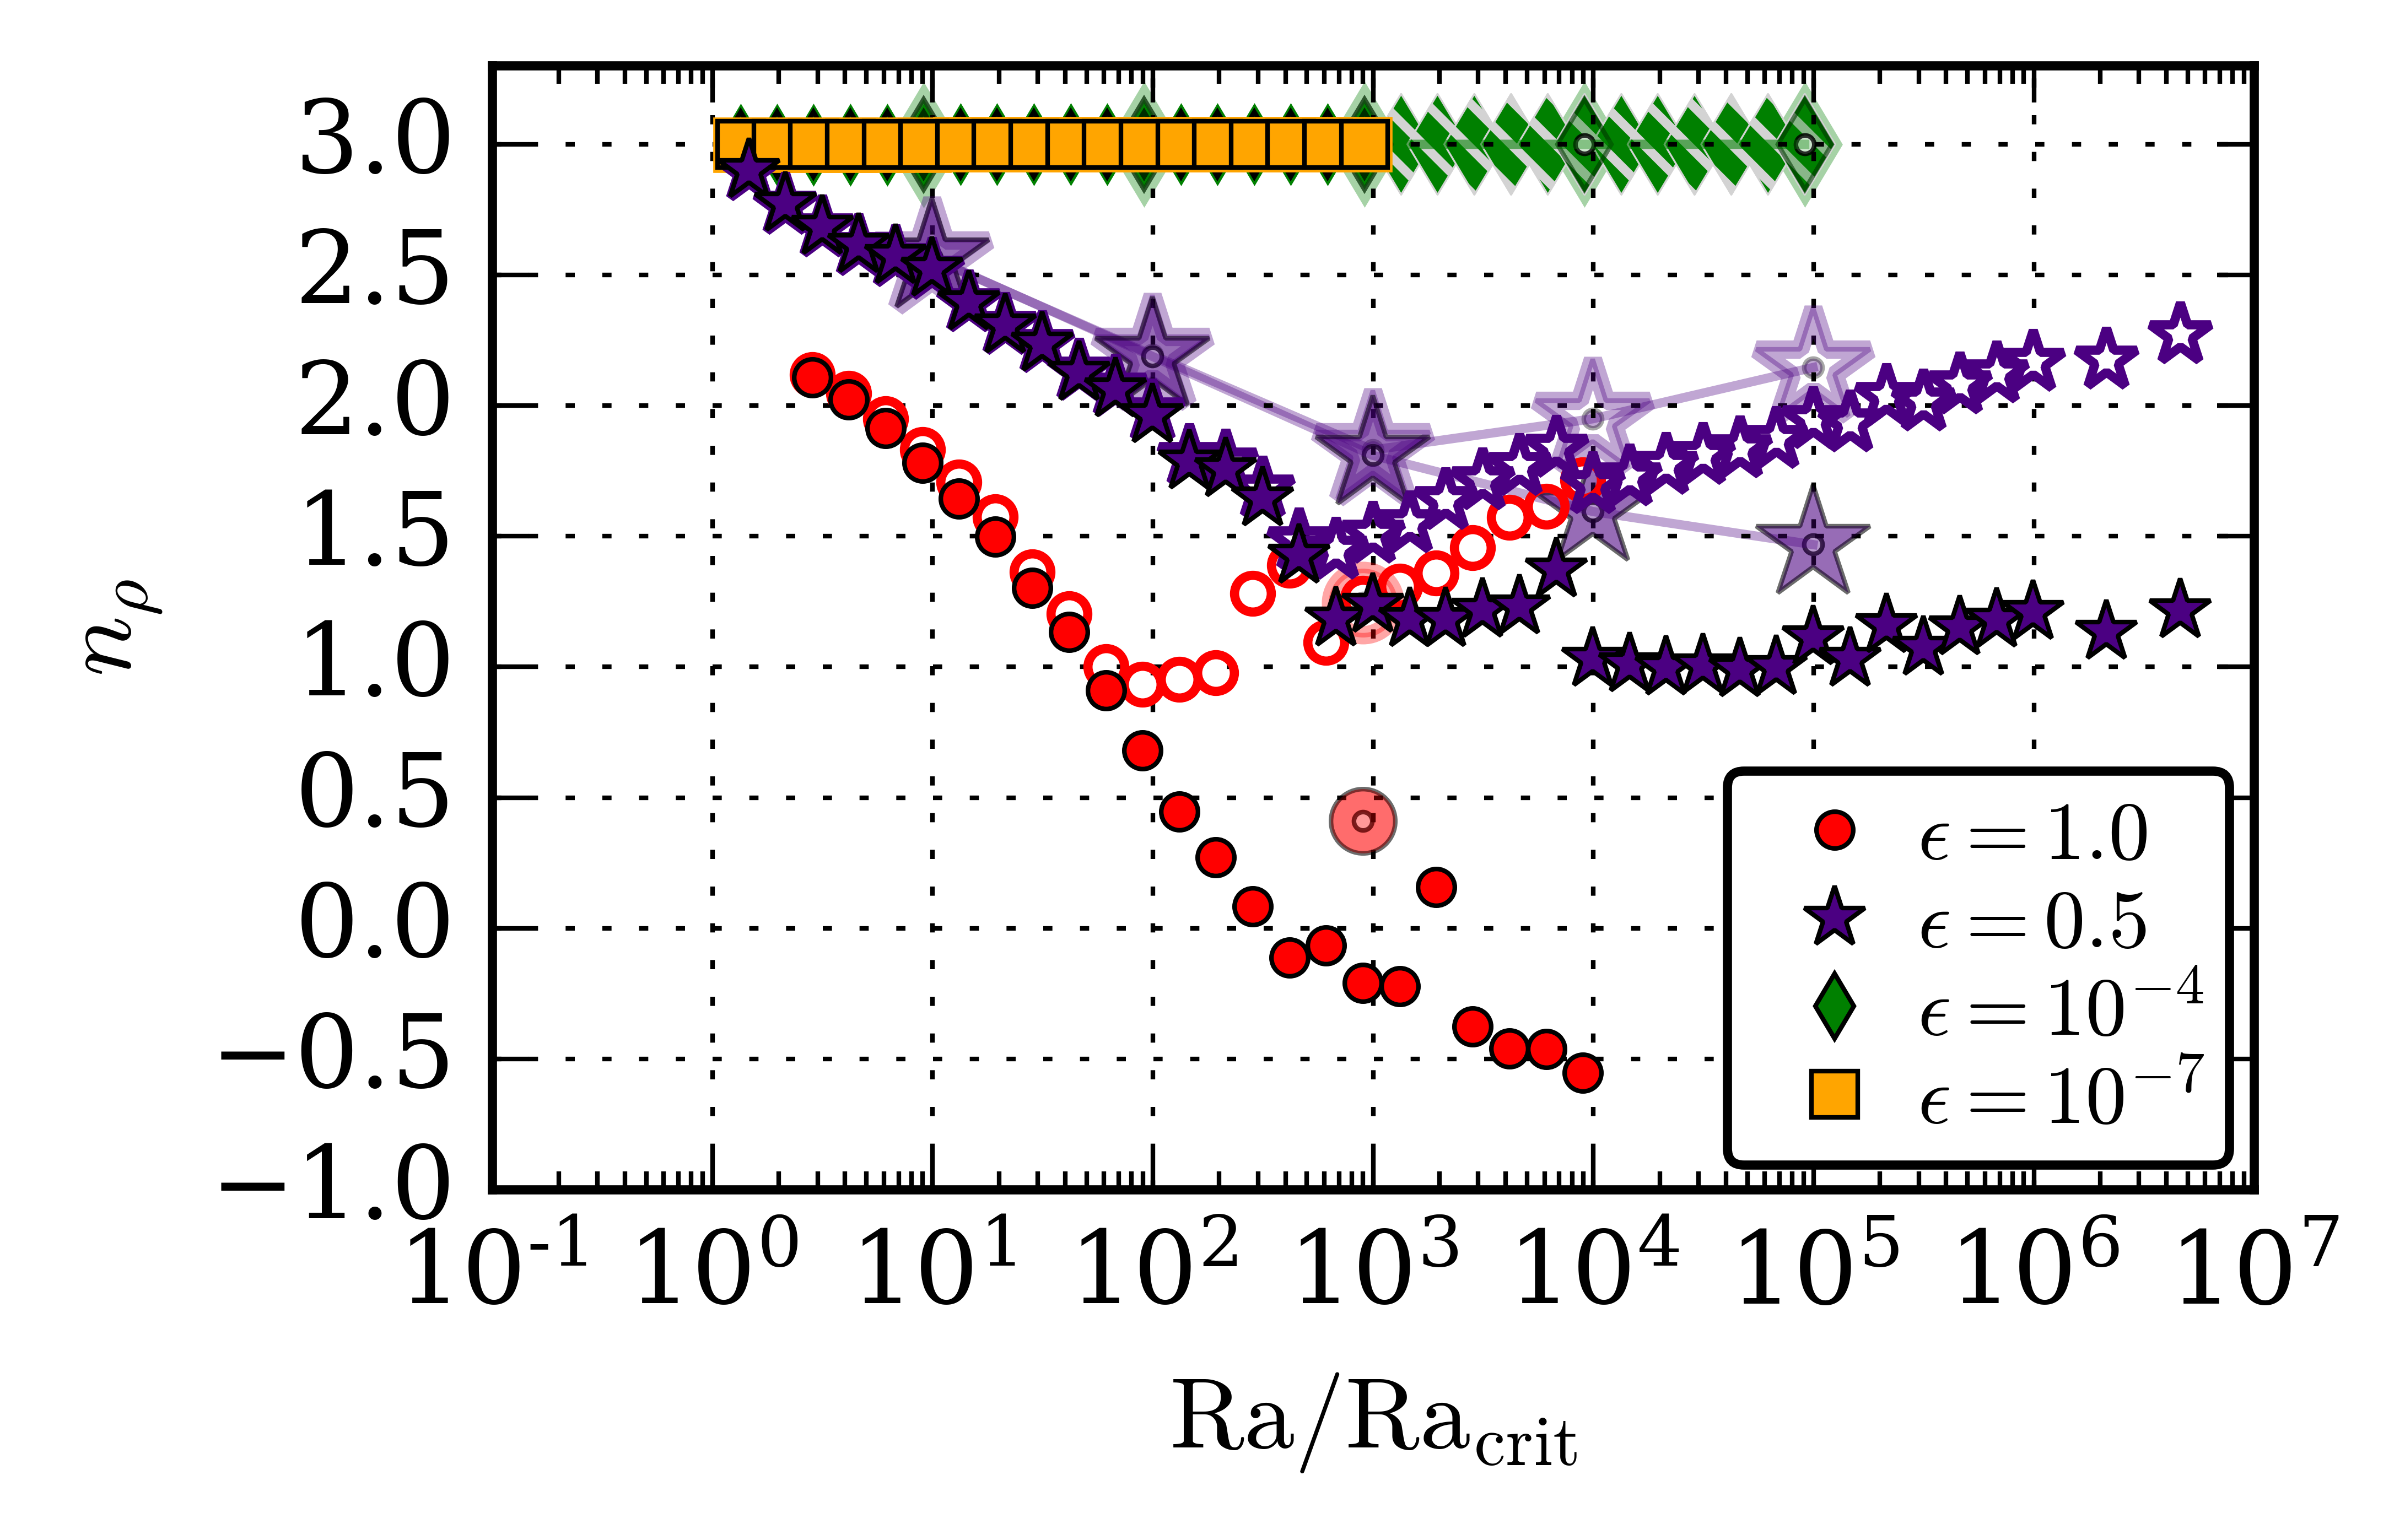
\includegraphics[width=3.4375in]{./figs/density_v_ra.png}
\caption{\label{fig:nrho_v_ra} We measure the stratification of 
evolved solutions
in two ways.  The solid symbols show $\ln(\rho(0)/\rho(L_z))$, 
or the density contrast
as measured at the upper and lower boundary.  The empty symbols show 
$\ln(\text{max}(\rho)/\text{min}(\rho))$. 
Unsurprisingly, at low $\epsilon$ the evolved
$n_{\rho}$ is not different from the initial conditions to first order.  
At high $\epsilon$,
the density contrast shrinks, and once the mean 
Ma approaches 1 the two methods of
measuring the density stratification bifurcate as density 
inversions form within the thermal
boundary layers.}
\end{figure}

As the thermodynamic variables converge to their steady state values, 
the density profile evolves while remaining in hydrostatic equilibrium 
to zeroth order.  In Fig. \ref{fig:nrho_v_ra} we show the number of density 
scale heights present in the evolved solution using two measures.  
We find that once the average Ma of the domain
becomes approximately one, large density inversions begin to 
form in the boundary layers, as was reported by \cite{brandenburg&all2005}.  
Regardless, the agreement of Nu across $\epsilon$, particularly at
low Ra, despite the difference in effective stratifications is striking.  

\section{Discussion}
\refstepcounter{section}
\label{sec:discussion}
In this letter we have studied fundamental heat transport by 
stratified convection in simplified 2-D polytropic atmospheres.
We argue that these atmospheres are the natural extension
of the RB problem to stratified systems, 
and are an ideal laboratory for understanding the basic 
properties of stratified convection. 
We see little difference between
the properties of our 2D and 3D results, which aligns with expectations
of Boussinesq theory and DNS results at values of Pr $\geq$ 1 \cite{ahlers&all2009}.

At low Ra and Ma, the scaling of Nu with Ra is reminiscent of RB convection.  
However, at high Ra and Ma, the scaling breaks down to a Ra$^{1/5}$ 
scaling unlike what is seen in Boussinesq convection.  
Similarly, the Reynolds number switches from a Ra$^{3/4}$ to
a Ra$^{1/2}$ scaling in this regime shift.  
It is interesting that both of these
scaling laws turn over by roughly a factor of 2/3.

Time-dependent oscillating shear states have developed spontaneously, 
as seen before in RB convection \cite{goluskin&all2014}.  
While computationally difficult, 
the highest values of Ra and the lowest value
of $\epsilon$ studied here are far from values found in nature.  
Future work will aim to better understand the mechanisms of shearing states and
whether or not these states are attainable in 
three-dimensional, non-rotating atmospheres. 

Furthermore, we have found that the stratification of 
these atmospheres evolves in a complex
manner, and future work should aim to 
understand the importance of changing stratification on
convective heat transport. Our studies
here will serve as a foundation both for understanding and 
comparing heat transport in stratified convection
to that in RB convection \cite{johnston&doering2009}, 
and for future studies of transport in stratified convection.  
These results can be used to determine if simplified equation sets, 
such as the anelastic equations, carry heat in the same manner as the 
FC equations.
This work will also be useful in coming to understand more realistic systems, 
such as rapidly rotating atmospheres \cite{julien&all2012},
atmospheres bounded by stable regions \cite{hurlburt&all1986}, 
or regions with realistic profiles of $\kappa$.



\subsection{acknowledgements}
EHA acknowledges the support of the University of Colorado's George 
Ellery Hale Graduate Student Fellowship.
This work was additionally supported by  NASA LWS grant number NNX16AC92G.  
Computations were conducted 
with support by the NASA High End Computing (HEC) Program through the NASA 
Advanced Supercomputing (NAS) Division at Ames Research Center on Pleiades
with allocations GID s1647 and GID g26133.
We thank Jon Aurnou, Axel Brandenburg, Keith Julien, Mark Rast, and Jeff Oishi 
for many useful discussions. We also thank the two anonymous referees whose
critical comments greatly improved the quality of this letter.

\bibliography{../biblio.bib}
\end{document}
